Automatic program synthesis has been a long term goal of the field of artificial intelligence since its inception \cite{mannaAutomaticProgramSynthesis1971}, promising to reduce the workload of software developers by automatically solving some of the tasks they face.
And since the field's inception it has been grappling with the challenging properties of the sparse optimization space \cite{alurSyntaxguidedSynthesis2013, davidProgramSynthesisChallenges2017} that is the set of all programs in a certain programming language, namely, 
\begin{enumerate}
    \item valid error-free programs constitute an exceedingly small part of the space of possible strings, so any program synthesis algorithm that incorporates random guessing (for instance, a randomly Reinforcement Learning with random initialization \cite{suttonReinforcementLearningSecond2018}) is exceedingly unlikely to guess a valid program.
    \item a small edit in a program can result in a large difference in it's behavior (and, conversely, the same algorithm can be expressed with very different programs), hence the programs we would like to find are not clustered in any compact part of the optimization space
    \item some of the evaluation mechanisms of programs, especially in the \emph{Programmatically Interpretable Reinforcement Learning} paradigm involve stochasticity and can yield different results for the same program.
\end{enumerate}

In other words, the search space in program synthesis is \emph{sparse}, \emph{brittle} and sometimes \emph{noisy} \cite{arnoldNoisyOptimizationEvolution2002} - all known challenges in Optimization Theory.

\section{Deductive methods}

One way to attack the sparsity of the search space is to look for hints in the task specification. 
Instead of (or in addition to) generating a program first and testing whether it adheres to specification, deductive methods apply equivalence rules to translate the specification into an executable 
This is hard to apply in \emph{Programmatically Interpretable Reinforcement Learning} where the specification is a black box, but can be a powerful approach in \emph{code translation} and \emph{programming by example} paradigms.

\newpage
\section{Evolutionary methods}

\begin{figure}[H]
    \centering
    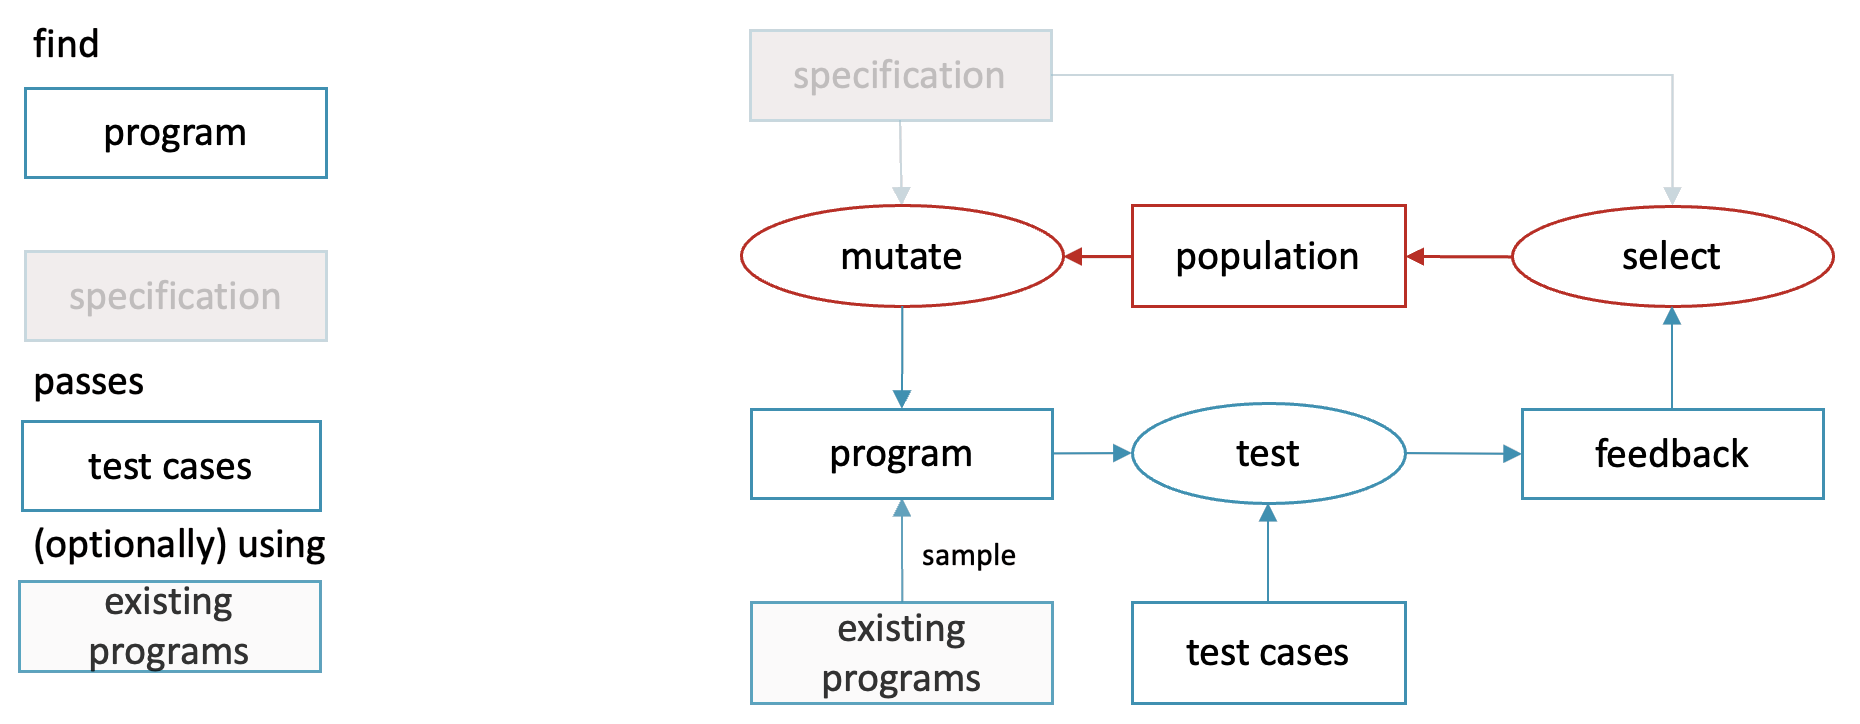
\includegraphics[width=\linewidth]{gp.png}
    \caption{Genetic Programming, schematic definition}
    \label{fig:gp}
\end{figure}

\newpage
\section{Constrained problem spaces}

\paragraph{Inductive logic programming}

\paragraph{Domain specific languages}

\paragraph{Grammar guided search}

\section{Pre-training methods}

\emph{Inductive synthesis}

\emph{concept space}

\paragraph{Autoencoder models}

\paragraph{Autoregressive models}

\section{Human in the loop}

\paragraph{Completion}

\paragraph{Sketching}

\section{Open problems}

Most open problems lie in the domain of \emph{Programmatically Interpretable Reinforcement Learning}

However, a fully autonomous system for Programmatically Interpretable Reinforcement Learning is yet to be devised. In chapter \ref{ch:bfpp}